\chapter{Results}\label{result}

This section will present the results of the circuits implemented in Chapter \ref{sec3}. We will examine both quantum simulator and quantum machine outputs and the effects of noise and interference on these outputs. We will be observing the QkNN circuit with the Wisconsin Breast Cancer data set \citep{BCWisconsinData} and the Iris dataset \citep{irisData}. For the Quantum Support Vector Mechanism and Grover's `search algorithm, we will observe their results using the Wisconsin Breast Cancer data set and the 3-SAT \citep{3SATData} problem, respectively.

We will then observe the influence of shot increase in relation to accuracy. Finally, we will inspect the runtime of quantum machine learning algorithms in comparison to their classical counterparts. 


\section{Understanding the Results}

As discussed in Section \ref{ERNoi}, errors, noise and interference have great effects on the outcome of a quantum process. This especially holds true with non simplistic circuits or circuits with greater depths. While we will not be observing the accuracy and the runtime of Grover's Search algorithm, we can observe the quantum simulation results using the 3-SAT input in Figure \ref{GrovRun}.  

%%%%%%%%%%%%%%%%%%%%%%%%%%%%%%%%%%%%%%%%
\begin{figure}[H]
      \centering
      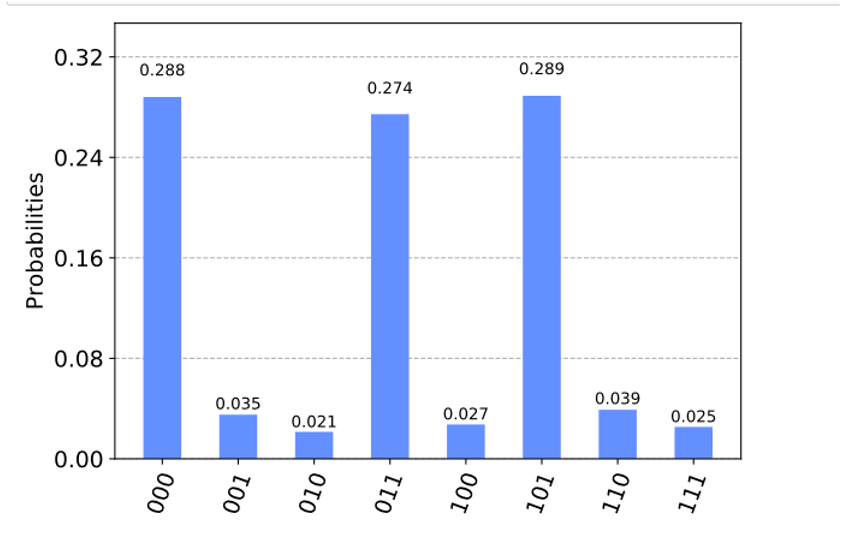
\includegraphics[scale=0.7]{background/Grovers.png}
      \caption{Grover's Search Algorithm results: 3-SAT Problem}
      \label{GrovRun}
\end{figure}
%%%%%%%%%%%%%%%%%%%%%%%%%%%%%%%%%%%%%%%%


Both Figure \ref{GrovRun} and Figure \ref{irisSim} are noise free quantum simulations, with the former depicting Grover's Search algorithm on the 3-SAT input and the latter depicting the Quantum k-Nearest Neighbour circuit applied to the Iris data set.

%%%%%%%%%%%%%%%%%%%%%%%%%%%%%%%%%%%%%%%%
\begin{figure}[H]
      \centering
      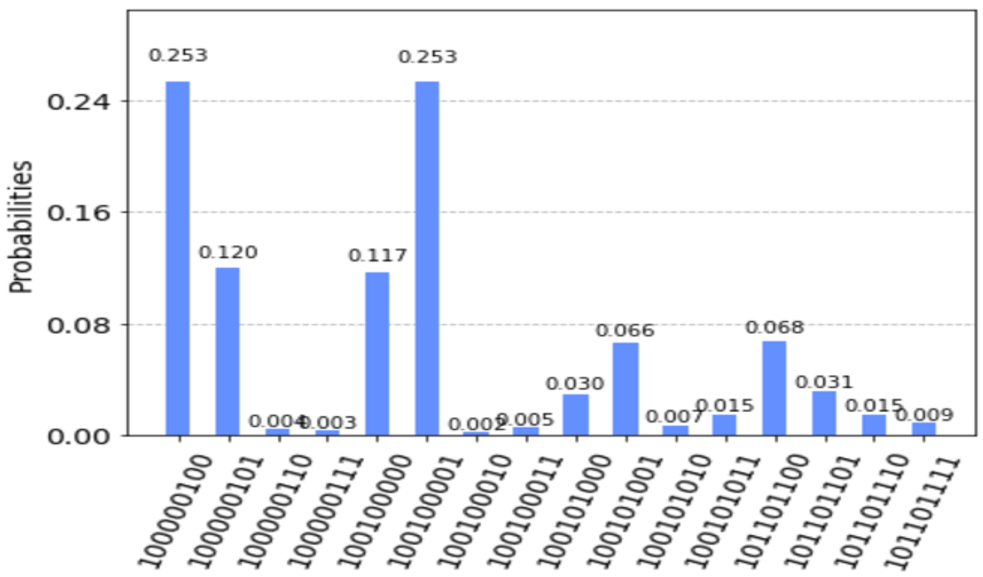
\includegraphics[scale=0.7]{background/IrisSimi.png}
      \caption{QkNN simulation results: Iris Dataset}
      \label{irisSim}
\end{figure}
%%%%%%%%%%%%%%%%%%%%%%%%%%%%%%%%%%%%%%%%


Figure \ref{IrisQuan} illustrates the circuit result using the same datasets on a (real) 15 qubit quantum computer. The bottom axis depicts all possible results and the y-axis details the probability of finding those results within the circuit. Those with similar probabilities can be grouped together and are ‘neighbours’. These probability groupings are easier to read and understand when viewing the quantum simulator output found in Figure \ref{irisSim}, than using the quantum machine output shown in Figure \ref{IrisQuan}. This is due to the output visualisation in Figure \ref{IrisQuan} encapsulating the noise, errors or gate inferences that may be present in our quantum circuit.


%%%%%%%%%%%%%%%%%%%%%%%%%%%%%%%%%%%%%%%%
\begin{figure}[H]
      \centering
      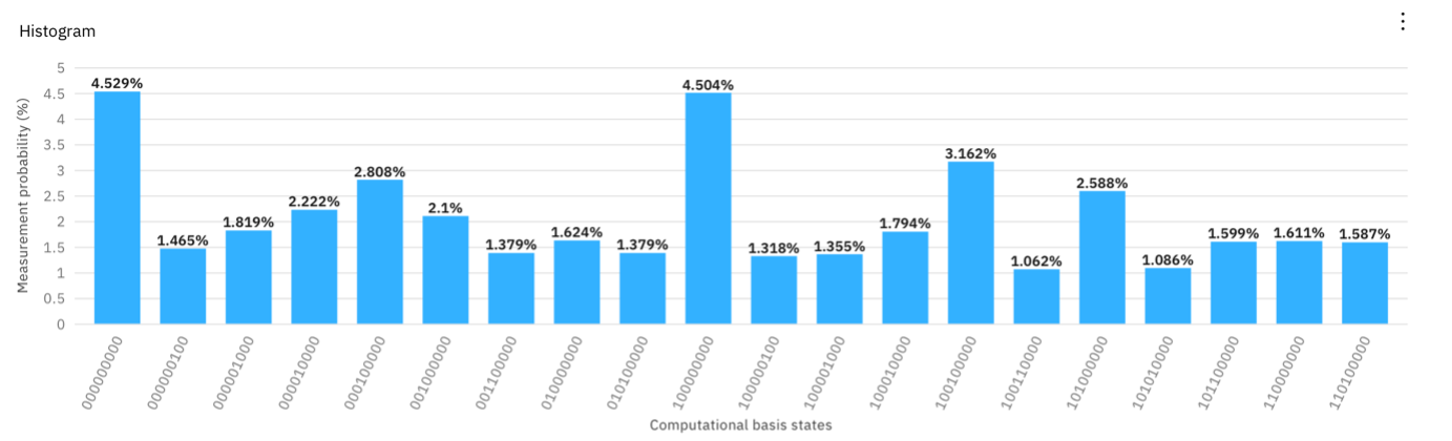
\includegraphics[scale=0.7]{background/irisQ.png}
      \caption{QkNN Quantum Run results: Iris Dataset}
      \label{IrisQuan}
\end{figure}
%%%%%%%%%%%%%%%%%%%%%%%%%%%%%%%%%%%%%%%%

\section{Shots and Accuracy}

In Section \ref{ERNoi} the use of shots in a quantum environment and its ability to reduce noise, interference and errors was discussed. While the reduction of these errors would theoretically increase an algorithm's accuracy, an increase in the number of shots does not necessarily retain in an increase in accuracy. Rather, it provides a more precise probability. This is because of errors such as gate interference, measurement errors, environmental noise and more, still exist within the device \citep{QiskitShots}. 



\begin{table}[H]
%\small
\caption{Quantum Machine Learning algorithms accuracy vs shots}
\label{tab:treatments}
\centering
\begin{tabular}{l l l l l l l}
\toprule
\textbf{No. of} & \textbf{QKNN} & \textbf{QKNN} & \textbf{kNN}& \textbf{kNN} & \textbf{QSVM} & \textbf{SVM}\\
\textbf{Shots} & \textbf{Iris} & \textbf{Breast}& \textbf{Iris} & \textbf{Breast} & \textbf{Breast}& \textbf{Breast}\\
\textbf{} & \textbf{} & \textbf{Cancer}& \textbf{} & \textbf{Cancer} & \textbf{Cancer}& \textbf{Cancer}\\
\textbf{} & \textbf{(\%)} & \textbf{(\%)}& \textbf{(\%)} & \textbf{(\%)} & \textbf{(\%)}& \textbf{(\%)}\\
\midrule
1 & - & - & 95 & 92 & - & 88\\
10 & 80 & 70& - & - & 72 & - \\
100 & 90 & 70 & - & - & 80 & -\\
1000 & 95 & 80& - & - & 87 & -\\
8192 & 95 & 80 & - & - & 89 & -\\
\bottomrule\\
\end{tabular}
\normalsize
\end{table}

%%%%%%%%%%%%%%%%%%%%%%%%%%%%%%%%%%%%%%%%
\begin{figure}[H]
      \centering
      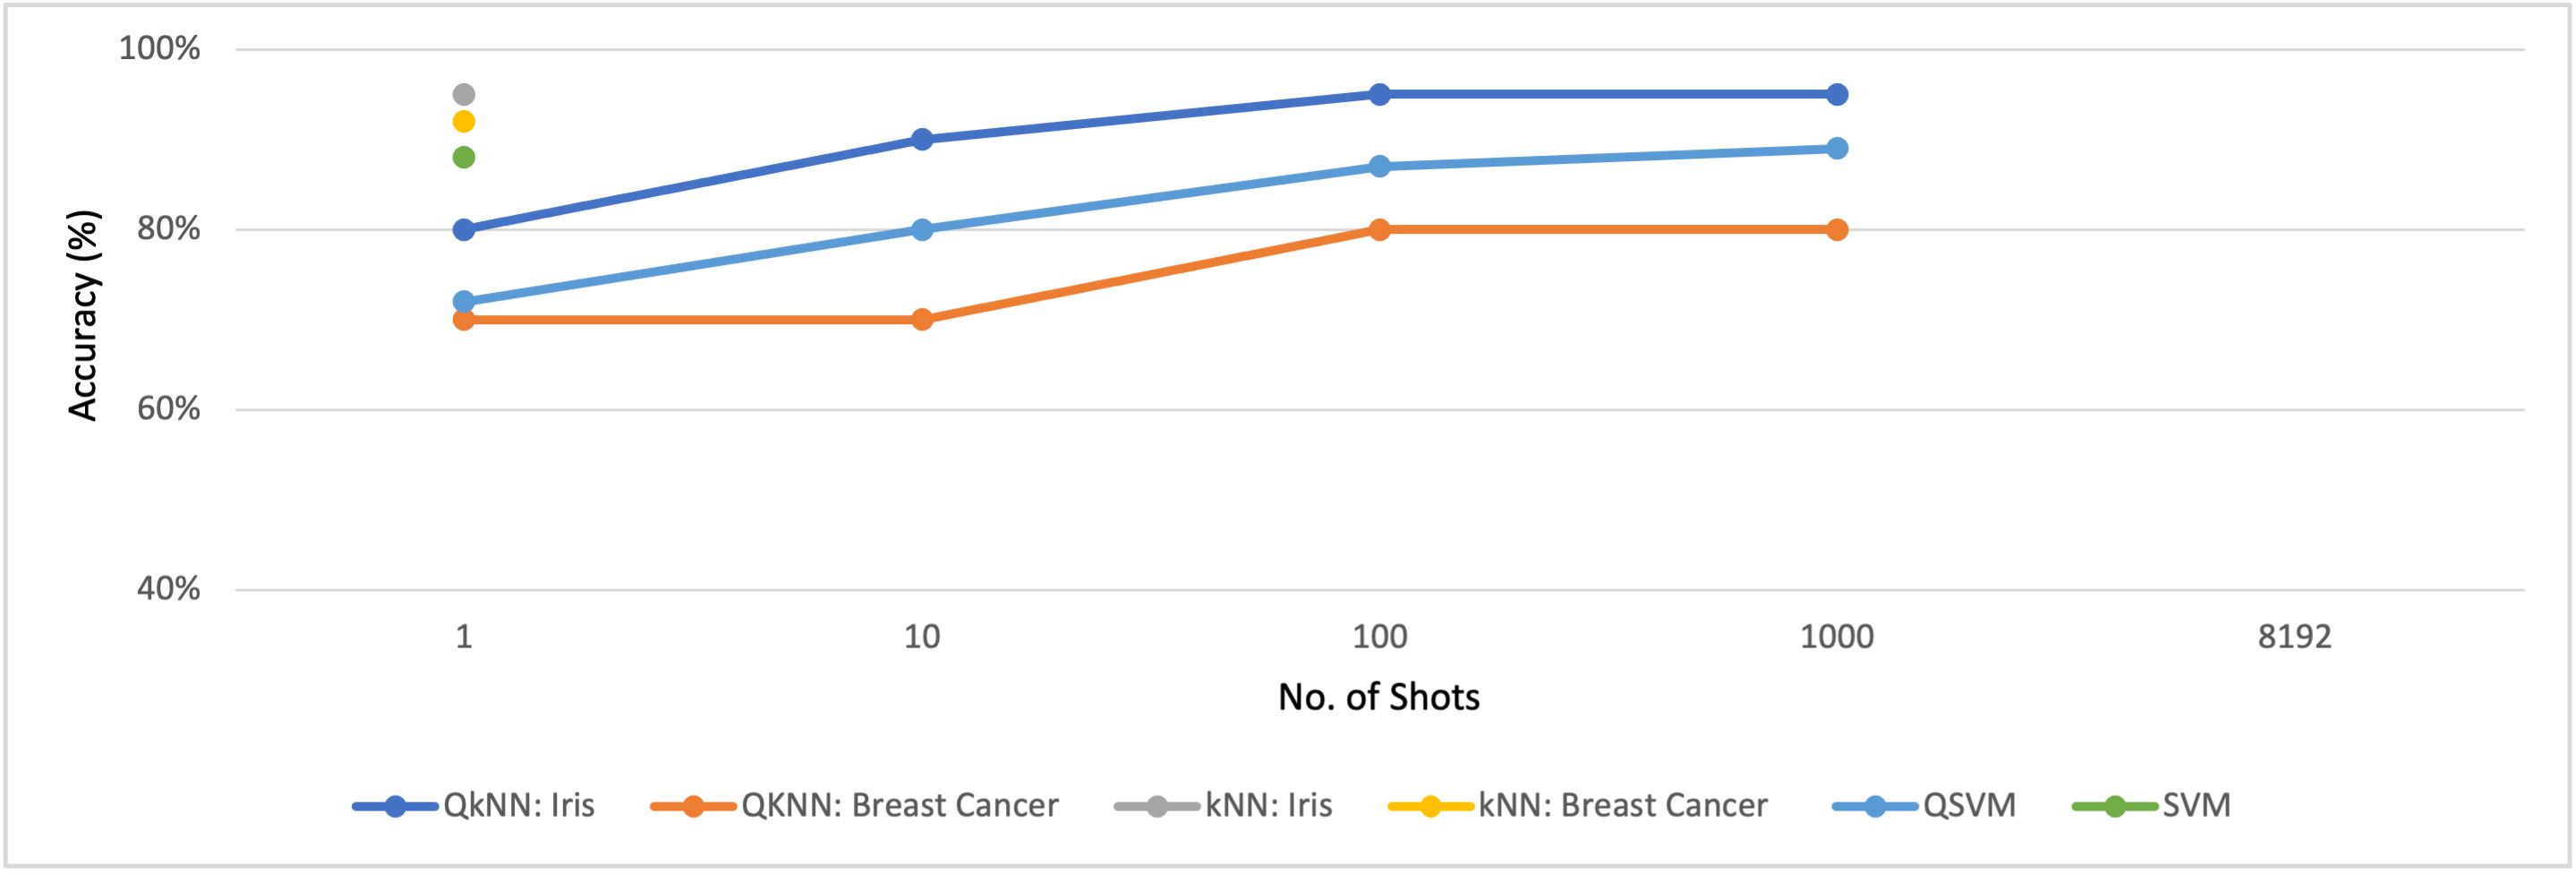
\includegraphics[scale=0.7]{background/accuracy.png}
      \caption{Quantum Machine Learning algorithms accuracy vs shots: Wisconsin Breast cancer and Iris datasets}
      \label{Accuracy}
\end{figure}
%%%%%%%%%%%%%%%%%%%%%%%%%%%%%%%%%%%%%%%%

In Figure \ref{Accuracy}, the resulting accuracy of each algorithm for the specified shot count may be seen. Of note, the dimensions are set to 100 for each dataset. The classical implementations were executed in a single shot, so they are represented as single dots in Figure \ref{Accuracy} and their multi-shot inputs are omitted from Table \ref{tab:treatments}. While an increase in the accuracy is seen, the quantum implementations do not surpass their classical counterparts. This is expected and can be attributed to various types of noise present in the quantum machine. 

\subsection{Shots and Runtime}
As discussed, circuit executions are repeated in order to confirm the probability that a qubit is in the state measured. Each repetition is called a \emph{shot}. With the circuit repeated multiple times, a question arises as to whether repetition affects circuit runtime. The Iris and the Breast Cancer datasets are used to evaluate this for the QSVM and QkNN circuits, with increasing shot counts of: 10, 100, 1,000 and 8,198 -- with 8,198 being the maximum number of shots available for the quantum machines available\footnote{The \texttt{quasi\_simulator} or the quantum simulator in Qiskit has a maximum shot count of 65,535.}. For this evaluation, the number of datapoints taken was fixed at 100.

\begin{table}
%\small
\caption{kNN and QkNN Shots vs Runtime}
\label{tab:treatments}
\centering
\begin{tabular}{l l l l }
\toprule
\textbf{No.} & \textbf{QkNN} & \textbf{QkNN} &  \textbf{QSVM} \\
\textbf{of} & \textbf{Iris} &  
\textbf{Breast} & \textbf{Breast}\\
\textbf{Shots} & \textbf{(seconds)} & \textbf{Cancer}& \textbf{Cancer}\\
\textbf{} & \textbf{} & \textbf{(seconds)}& \textbf{(seconds)}\\
\midrule
10 & 10.6 & 10.9 & 92  \\
100 & 12.2 & 11.2 & 107 \\
1000 & 16.7 & 16.2 & 164 \\
8192 & 52.2 & 52.5 & 878 \\
\bottomrule\\
\end{tabular}
\normalsize
\end{table}

%%%%%%%%%%%%%%%%%%%%%%%%%%%%%%%%%%%%%%%%
\begin{figure}[H]
      \centering
      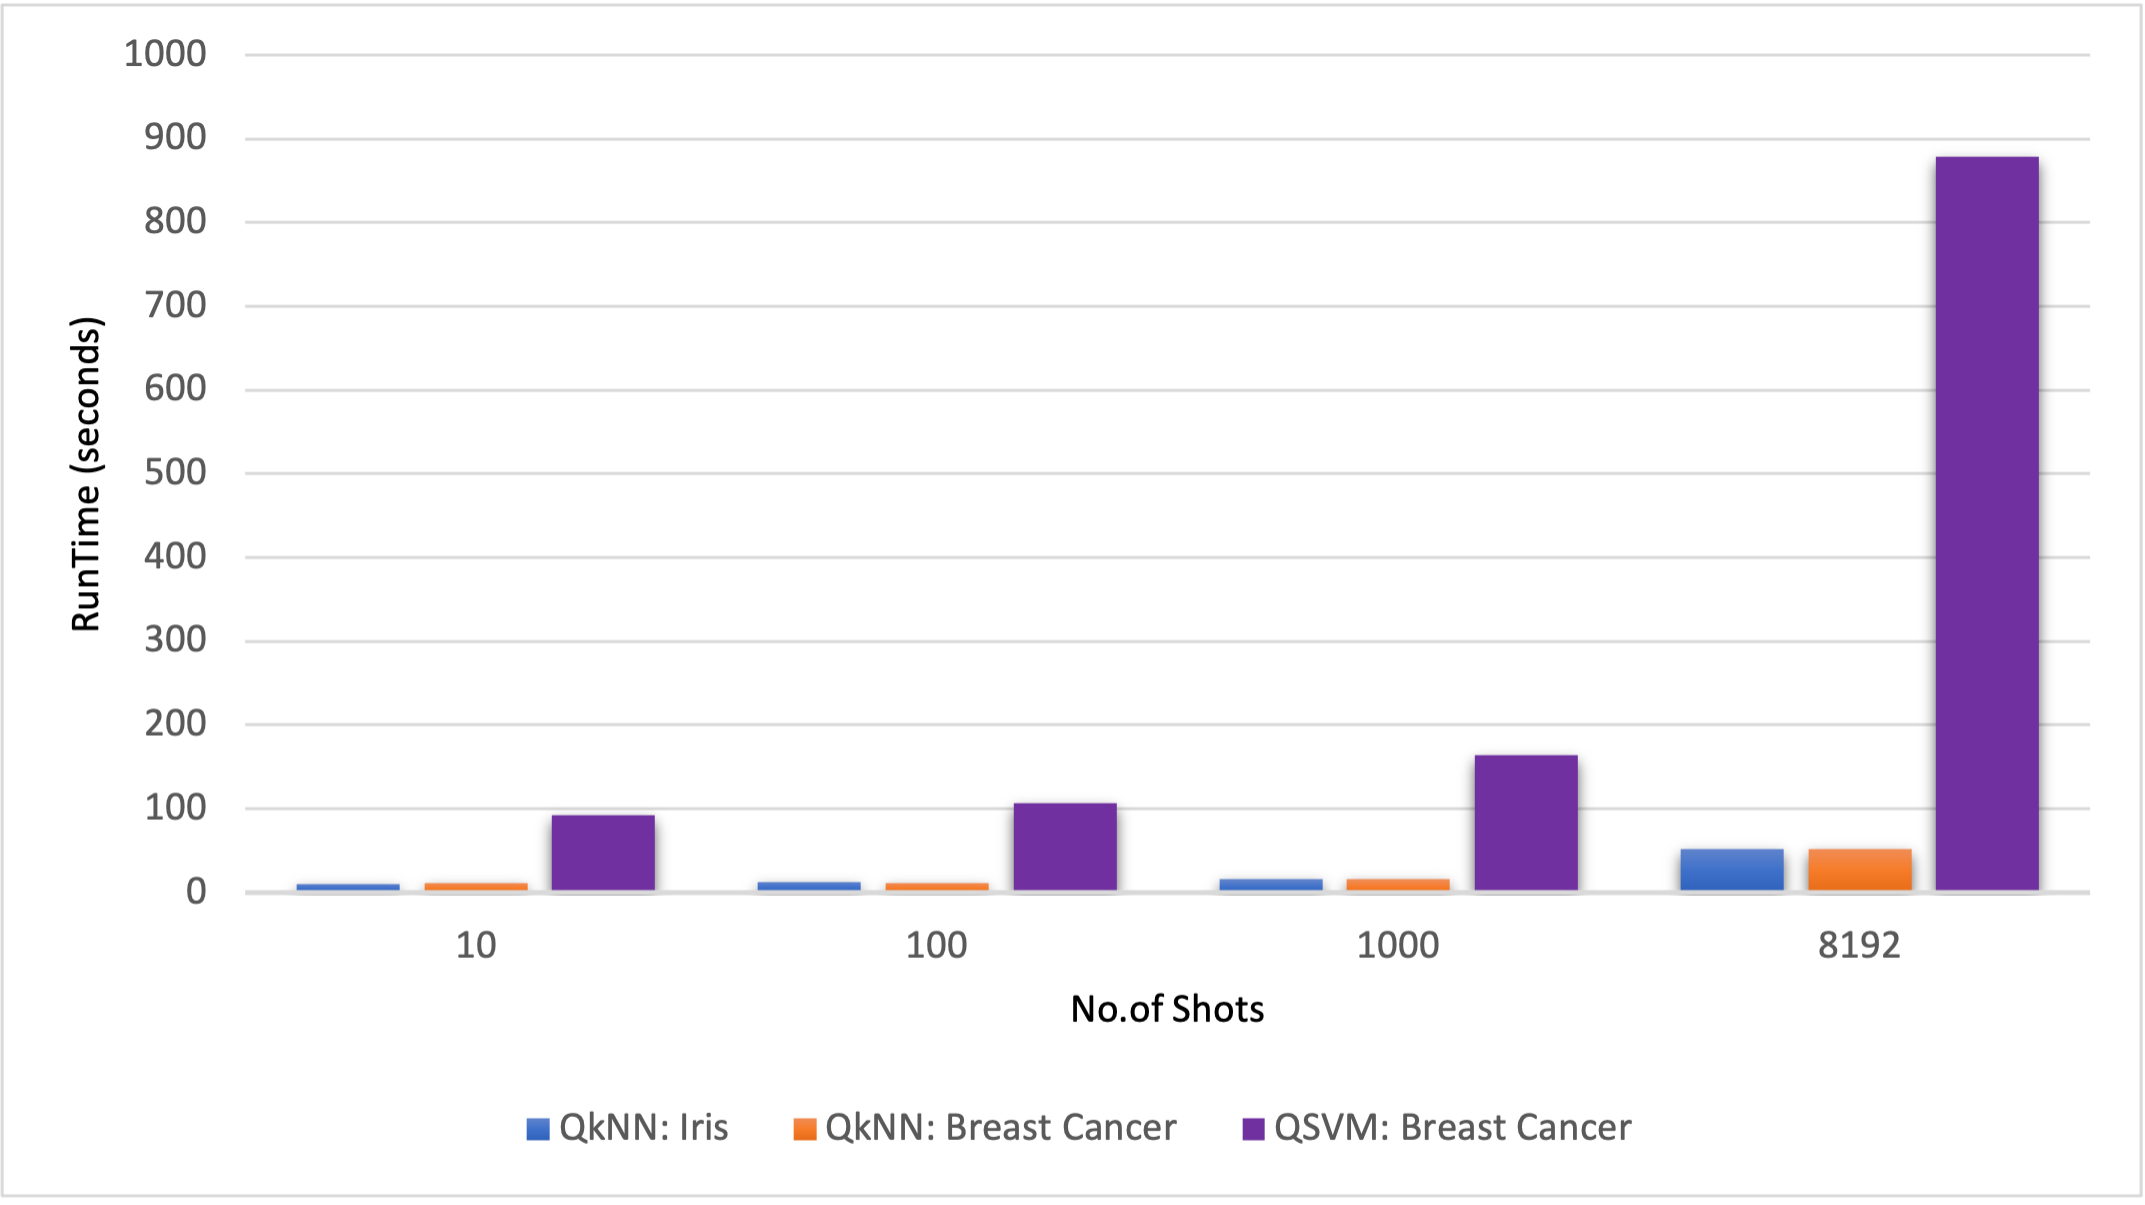
\includegraphics[scale=0.7]{background/shotsVsRun.png}
      %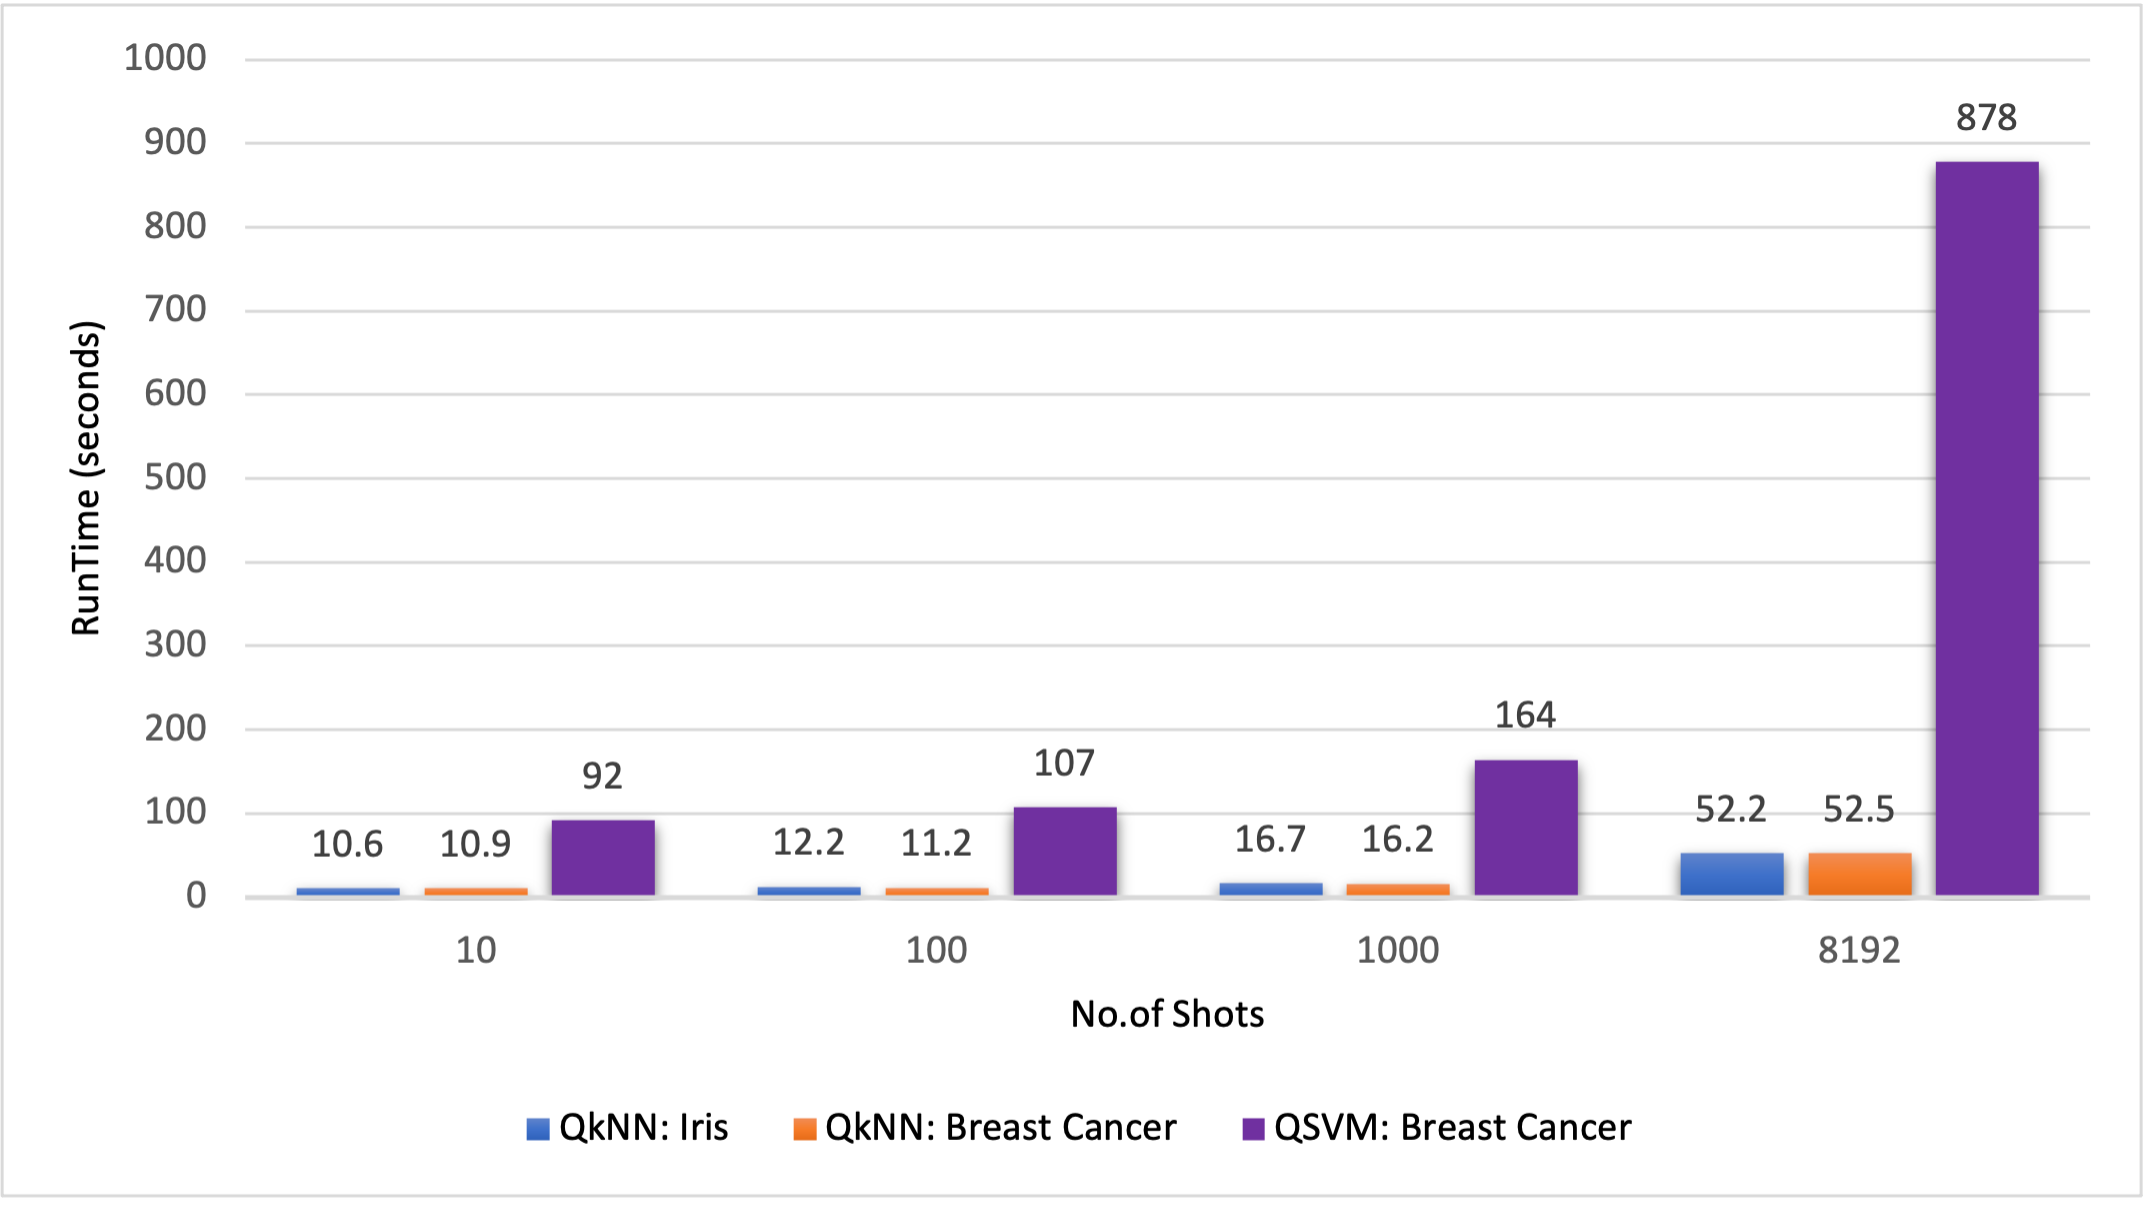
\includegraphics[scale=0.7]{background/ShotsValues.png}
       %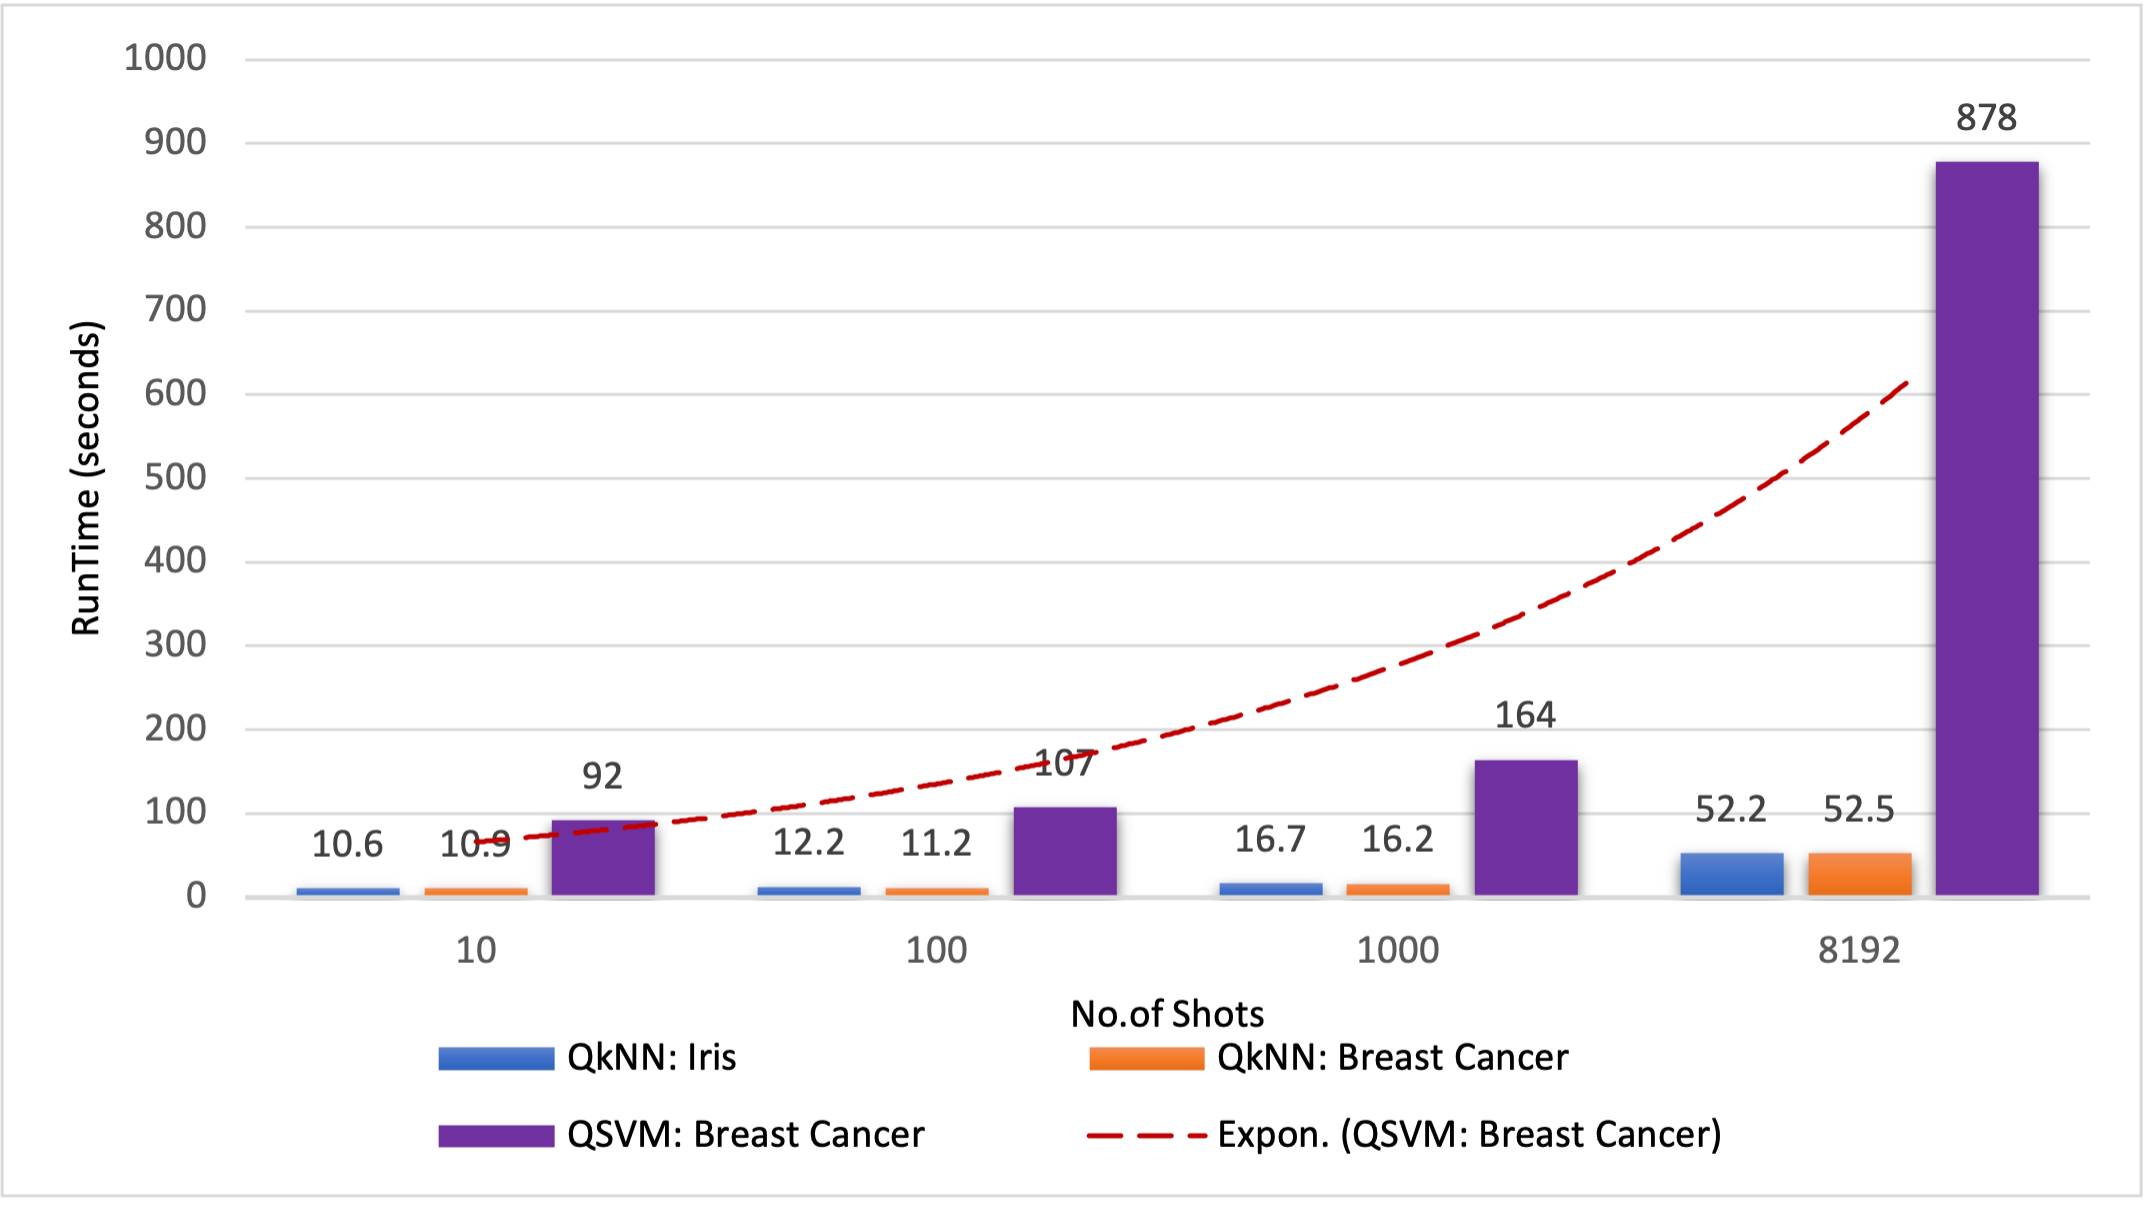
\includegraphics[scale=0.7]{background/ShotsWithLinearLine.png}
      \caption{kNN and QkNN Shots vs Runtime}
      \label{ShotVRun}
\end{figure}
%%%%%%%%%%%%%%%%%%%%%%%%%%%%%%%%%%%%%%%%
Figure \ref{ShotVRun} shows that an increase in the shot count causes an increase in the runtime.
% the x = no of shots
% y = runtime 
% if proportional, you get a straight time ( linear)

% Put numbers in agraph 



\section{Runtime}\label{RuntimeOut}
To truly test the proposed advantage of quantum computers, the execution time for both QkNN and QSVM in our datasets must to compared to their classical versions. We do so by increasing the data points or dimensionality of the input. 

The Breast Cancer dataset and the Iris dataset used have maximum data points of 569 and 150 respectively. In Figure \ref{kNNRunT}, we can see the runtime results for the QkNN circuit with the dimensions 10, 100, 150 and 500 data points for the Breast Cancer and Iris datasets. Figure \ref{kNNRunT} shows the clear quantum advantage of QkNN.

\begin{table}
%\small
\caption{kNN and QkNN Runtime vs Dimensions}
\label{tab:treatments}
\centering
\begin{tabular}{l l l l  l}
\toprule
\textbf{Dimensions} & \textbf{QkNN}& \textbf{kNN} & \textbf{QkNN} &  \textbf{kNN} \\
\textbf{} & \textbf{Iris} & \textbf{Iris} &  
\textbf{Breast} & \textbf{Breast}\\
\textbf{} & \textbf{(minutes)} &  \textbf{(minutes)} & \textbf{Cancer}& \textbf{Cancer}\\
\textbf{} & \textbf{} &  \textbf{} &  \textbf{(minutes)}& \textbf{(minutes)}\\
\midrule
10 & 1.1061 & 13.32 & 2.013 &  2.09 \\
100 & 1.35 & 15.98 & 2.1545 & 3.97\\
150 & 1.512 & 23.48 & 2.398 & 5.89\\
500 & 1.763 & - & 2.525 & 19.83\\
\bottomrule\\
\end{tabular}
\normalsize
\end{table}
%%%%%%%%%%%%%%%%%%%%%%%%%%%%%%%%%%%%%%%%
\begin{figure}[H]
      \centering
      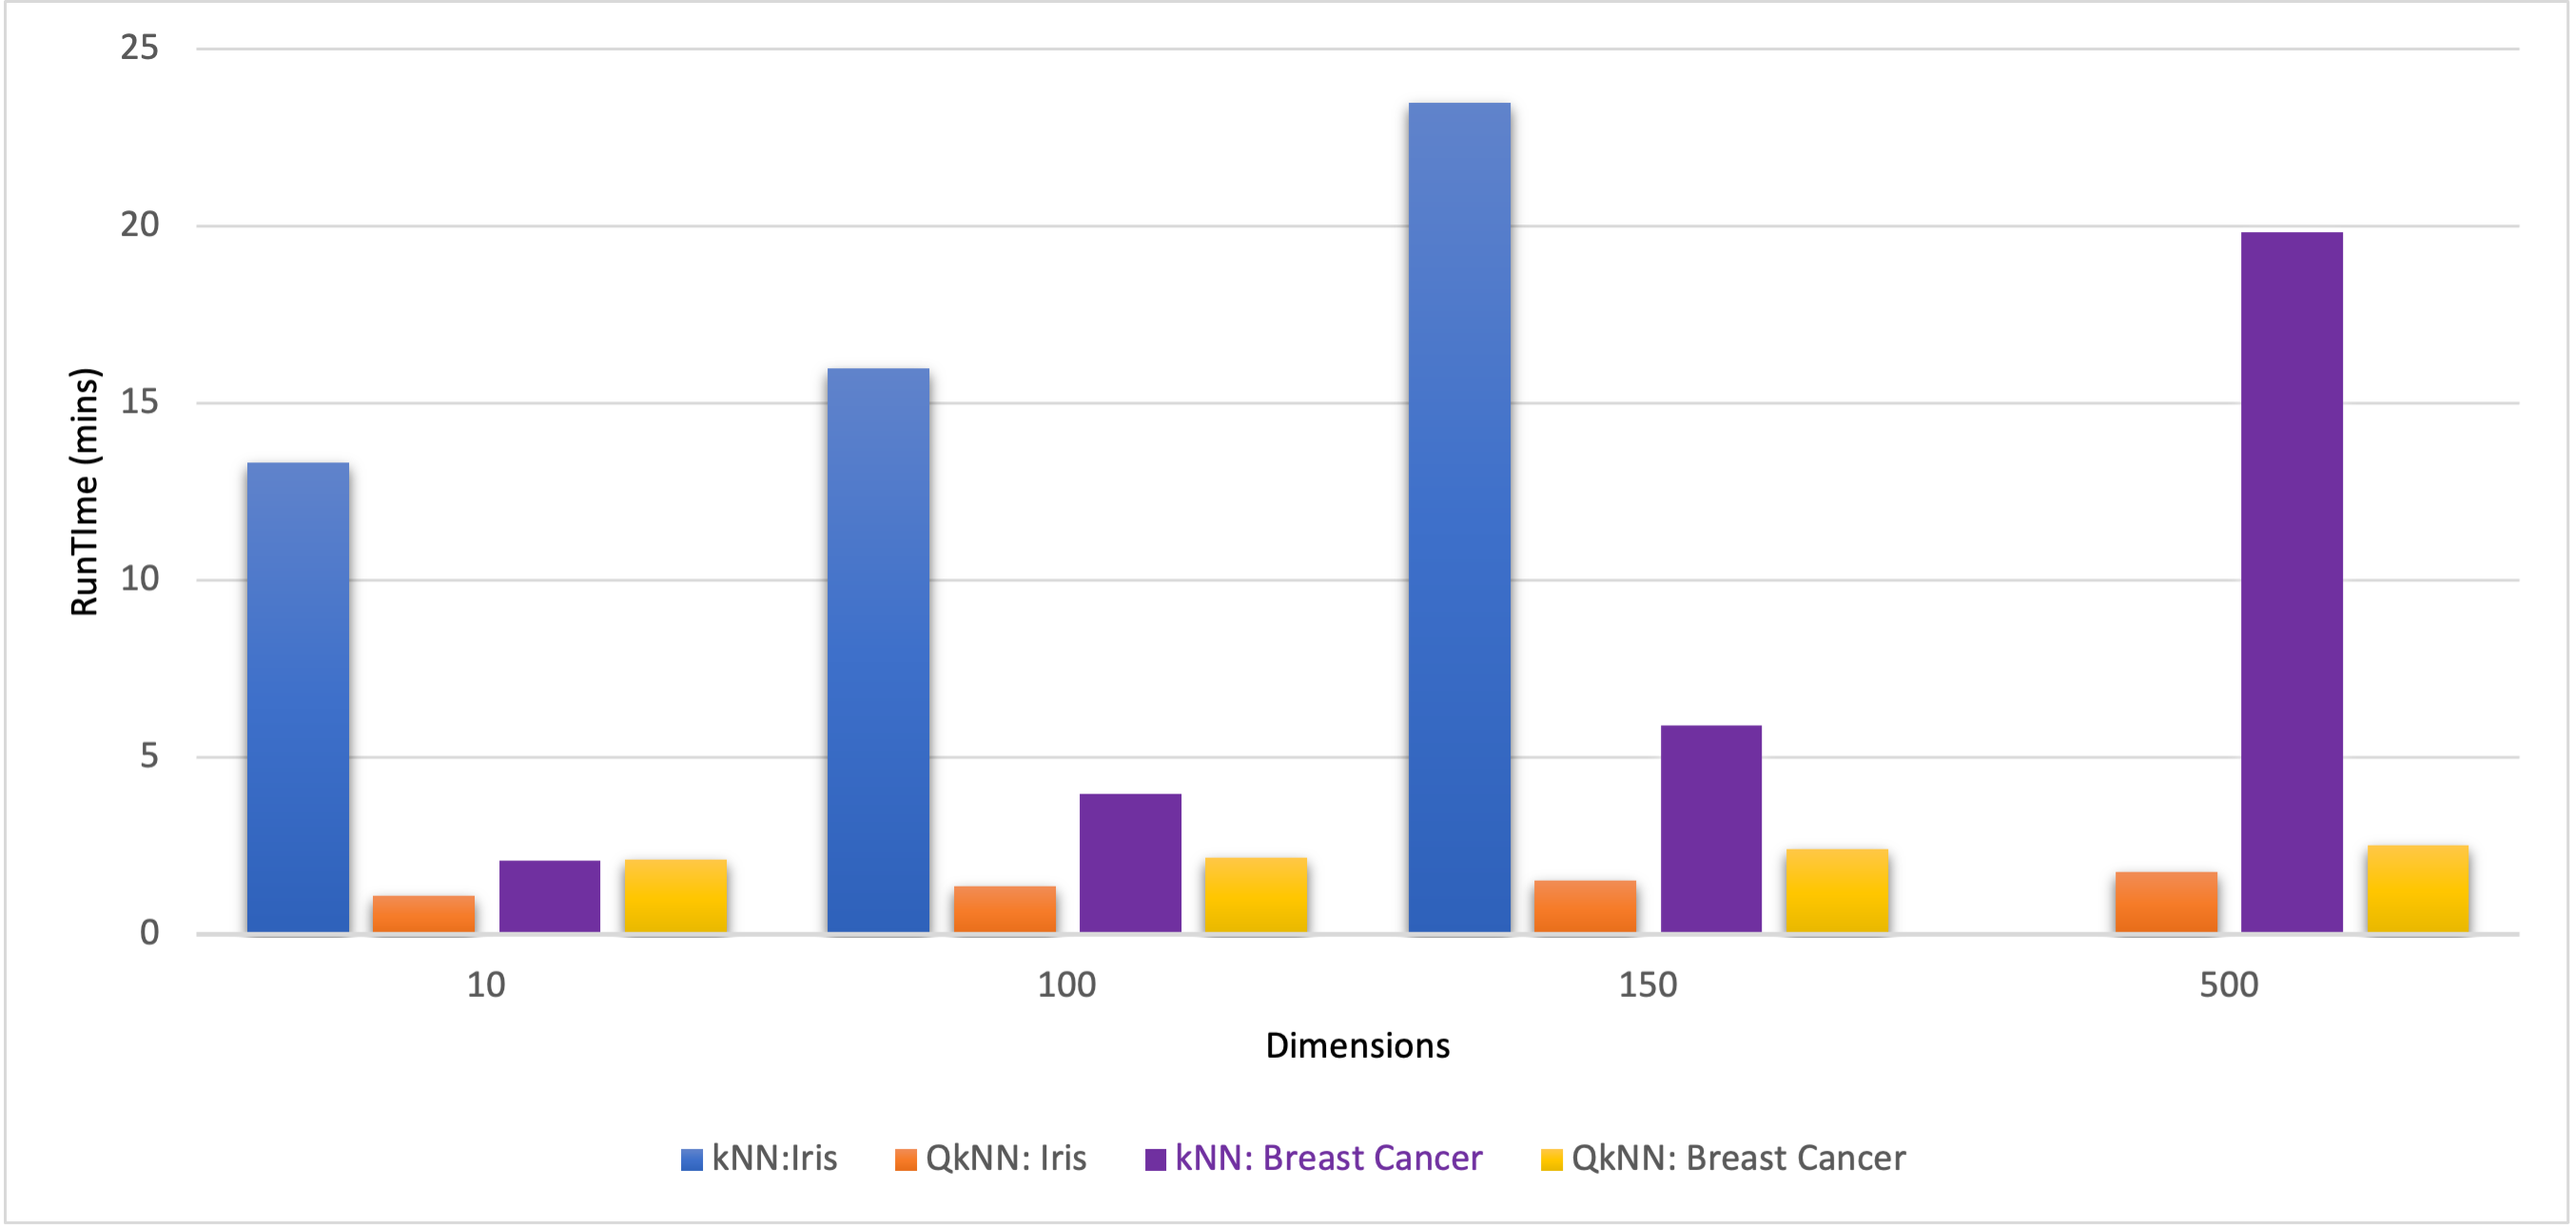
\includegraphics[scale=0.7]{background/KnnRun2.png}
      \caption{kNN and QkNN Runtime vs Dimensions: Wisconsin Breast cancer and Iris datasets}
      \label{kNNRunT}
\end{figure}
%%%%%%%%%%%%%%%%%%%%%%%%%%%%%%%%%%%%%%%%

The QSVM dimensions for the Breast Cancer dataset were 10, 50 and 150. Figure \ref{SVMRunT} illustrates that 
the QSVM algorithm saw a little increase in speed. Overall it was surprisingly comparable to the SVM implementation. 


\begin{table}
%\small
\caption{SVM and QSVM Runtime vs Dimensions}
\label{tab:treatments}
\centering
\begin{tabular}{l l l }
\toprule
\textbf{Dimensions} & \textbf{QSVM}& \textbf{SVM} \\
\textbf{} & 
\textbf{Breast} & \textbf{Breast}\\
\textbf{} & \textbf{Cancer}& \textbf{Cancer}\\
\textbf{} & \textbf{(minutes)}& \textbf{(minutes)}\\
\midrule
10 & 3.2 & 3.17 \\
50 & 4.58 & 4.5 \\
150 & 4.57 & 5.89 \\

\bottomrule\\
\end{tabular}
\normalsize
\end{table}

%%%%%%%%%%%%%%%%%%%%%%%%%%%%%%%%%%%%%%%%
\begin{figure}[H]
      \centering
      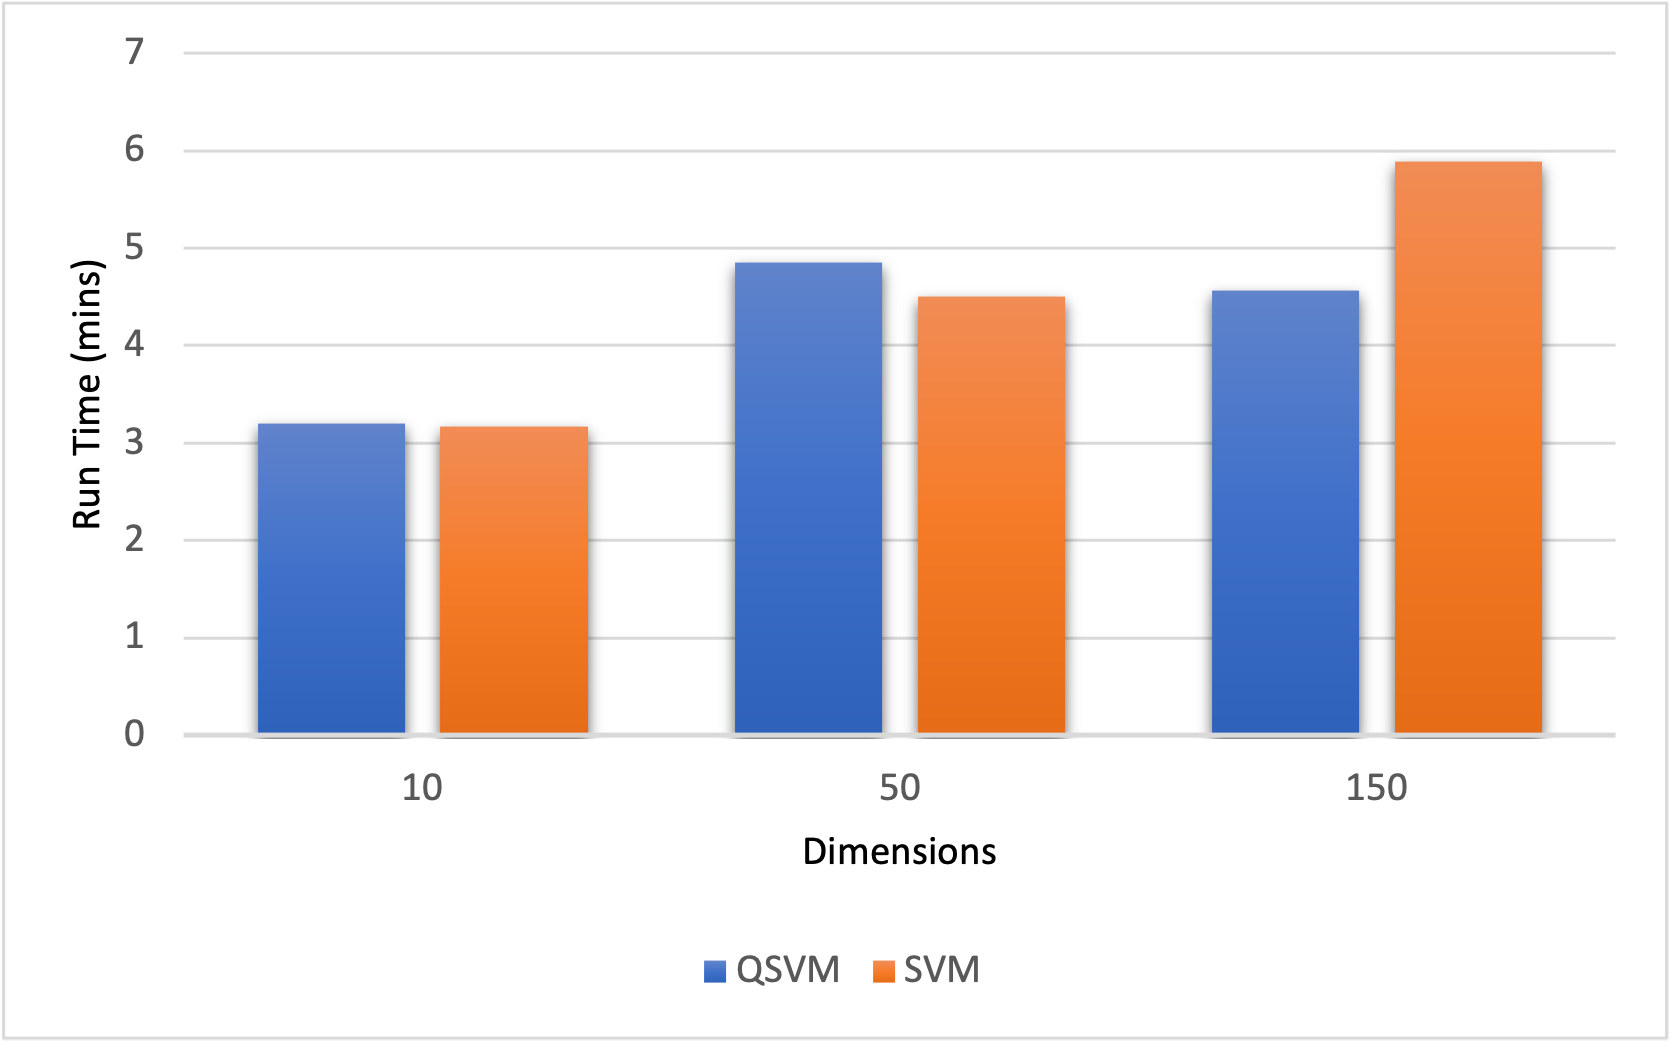
\includegraphics[scale=0.8]{background/SVMRunT.png}
      %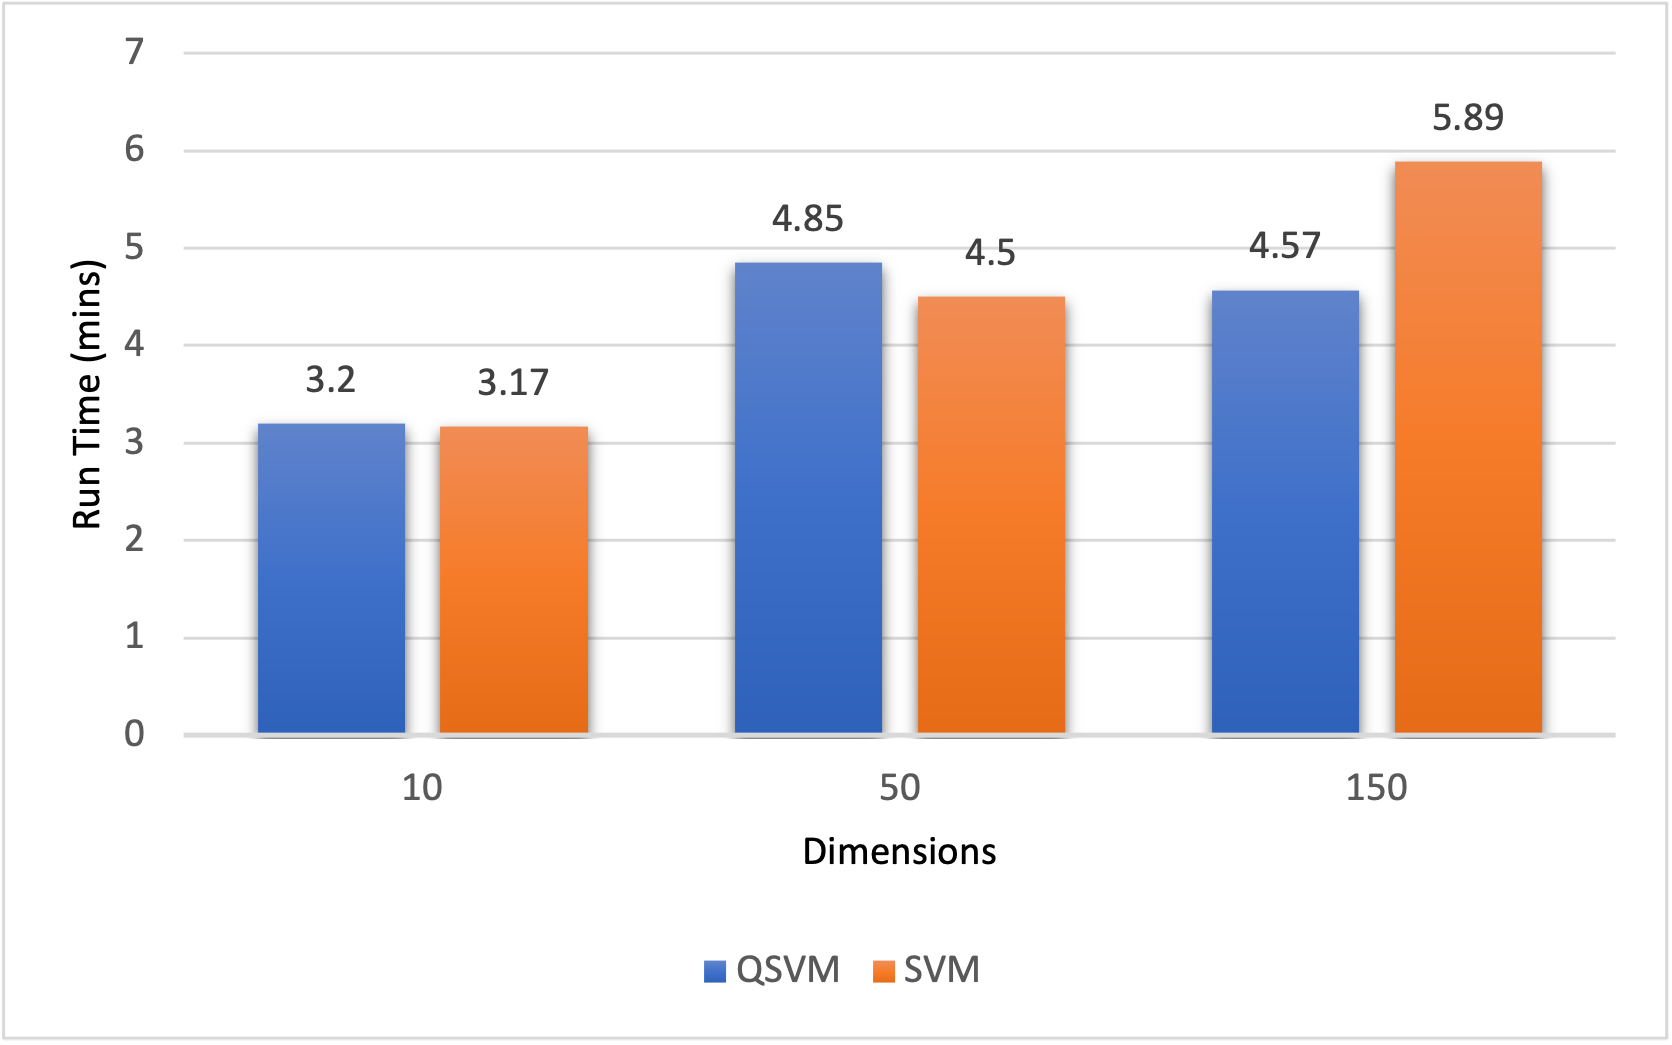
\includegraphics[scale=0.8]{background/RSVMValues.png}
      \caption{SVM and QSVM Runtime vs Dimensions: Wisconsin Breast cancer dataset}
      \label{SVMRunT}
\end{figure}
%%%%%%%%%%%%%%%%%%%%%%%%%%%%%%%%%%%%%%%%

However, the QkNN circuit highlights the proposed advantage of quantum computers. We can see that the runtime results from QkNN shadow that of kNN. To note, when running a quantum system, the queue time can be long but the transplaining and execution time is mere seconds. 
